\chapter{Analytical Needle Probe Approach}
\label{sec:analytical-np}
\bigskip

\section{Introduction}
\label{sec:analytical-np:intro}

The technique used to measure thermal conductivity with a needle probe is based
on the assumption that the needle approximates an infinite line source of energy
with a constant heat flux embedded in an infinite medium. The origins of the
analytical solution for isotropic thermal conductivity may be found in Carslaw
and Jaeger's book, ``Conduction of Heat in Solids.'' \cite{basictheory}

The method based on Carslaw and Jaeger's solution depends on solving a 2-D
problem, where all planes orthogonal to the needle have the same temperature
distribution; in other words, temperature is not a function of axial position.
Moreover, the problem is further simplified by posing the problem into radial
coordinates and solving for temperature as a function of radial distance only.

In the isotropic case, this is straightforward, as conductivity is a constant
scalar. Unfortunately the anisotropic case is more complex, but luckily not
completely intractible.

\section{The Isotropic Case}
\label{sec:analytical-np:isotropic}

The isotropic case solves the following equation:

\begin{equation*}
-k\nabla^2 T = \rho C\frac{\partial T}{\partial t}
\end{equation*}

Where \(T\) is temperature, \(k\) is a scalar thermal conductivity, \(\rho\) is
density, \(C\) is volumetric heat capacity, and \(t\) is time.

\marginpar{From Carslaw \& Jaeger, pg. 261}

By casting this problem into cylindrical coordinates, the equations may be
simplified such that they are a function of radial distance \(r\) only (as
temperature is assumed to not be a function of axial position \(z\) or angle
\(\phi\)).

After applying this transformation and solving the equation, the analytical
solution to the problem becomes:

\begin{equation}
\label{isotropic_ei}
T(r,t) = - \frac{q}{4\pi k}\Ei\left(-\frac{r^2}{4kt}\right)
\end{equation}

where \(q\) is heat flux from the needle per linear distance, and \(\Ei()\) is
as defined in equation \ref{eq:ei} for real-valued arguments.

\begin{equation}
\label{eq:ei}
\Ei(x) = -\int_{-x}^{\infty} \frac{e^{-t}}{t}dt
\end{equation}

Solving for the exponential integral analytically is not possible, and numerical
solutions can be difficult. Typically, we instead use an approximation for small
\(r/t\),

\begin{equation}
\label{isotropic_case}
T(r,t) = \frac{q}{4\pi k}\ln\left(\frac{4kt}{r^2}\right) - \frac{\gamma q}{4\pi k}
\end{equation}

Typical use of this function is to find \(\frac{dT}{d(\ln t)}\) and solve
for \(k\). We will be working with Equation \ref{isotropic_case} for the remainder of
this analysis, though it could easily be applied to \ref{isotropic_ei} as well.


\section{Difficulties In The Anisotropic Case}
\label{sec:analytical-np:anisotropic-diff}


The anisotropic case varies from the isotropic one in that instead of a scalar 
thermal conductivity \(k\), one must solve the problem using an \(n \times n\)
thermal conductivity, \([K]\), where \(n\) is the number of dimensions in the
problem. As a consequence, reducing the problem into two dimensions becomes more
difficult. Moreover, when the problem is posed in cylindrical coordinates, the
solution becomes a function not only of \(r\), but of \(\phi\) as well.

\section{Posing The Problem in Two Coordinates}
\label{sec:analytical-np:2D}

By assuming that temperature distribution is not a function of axial direction
\(z\), we may reduce the problem to an analogous one in orthogonal directions
\(x\) and \(y\) instead:

\begin{equation}
-\nabla_{xy} \cdot \left([K]_{2 \times 2}\nabla_{xy} T \right)= \rho C\frac{\partial T}{\partial t}
\end{equation}

Without loss of generality, it may be further simplified like so:

\begin{equation}
-\nabla \cdot \left(\begin{bmatrix}k_x & 0\\ 0 & k_y\end{bmatrix}\nabla T \right)= \rho C\frac{\partial T}{\partial t}
\end{equation}

We are able to do this by choosing the directions \(x\) and \(y\) such that the
matrix is diagonal.

The values of \(k_x\) and \(k_y\) may be found by finding the components of
\([K]\) that are in the \(xy\) plane, as illustrated in figure \ref{fig:projection}. 
In particular, equation \ref{eq:projection} was used in practice.

\begin{equation}
\label{eq:projection}
\left[ k_x, k_y \right] = 
\Eig\left(\begin{bmatrix} 1 & 0 & 0 \\ 0 & 1 & 0\\ 0 & 0 & 0\end{bmatrix}
\left[K\right]\right)
\end{equation}

\begin{comment}
\begin{figure}[h]
\centering
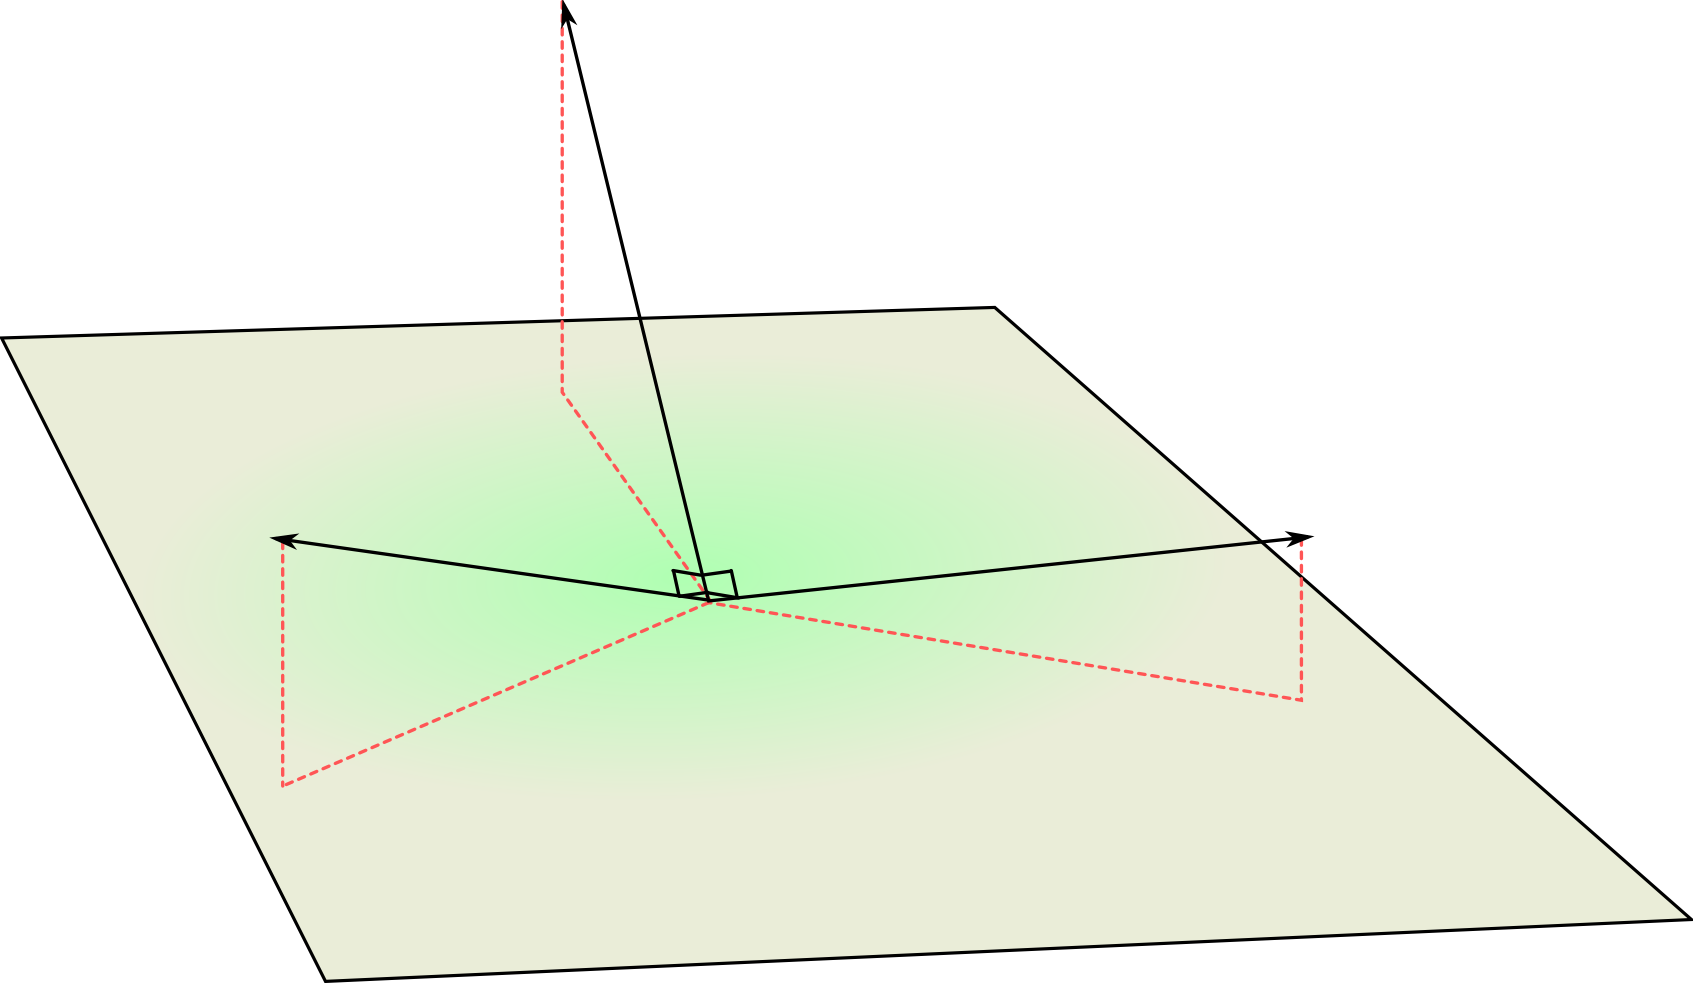
\includegraphics[width=0.6\textwidth]{fig/projection.png}
\label{fig:projection}
\caption{An informal demonstration of how the 3-D problem may be projected onto a 2-D domain.}
\end{figure}
\end{comment}

\section{Coordinate Transformation}
\label{sec:analytical-np:transformation}

\begin{figure}[h]
\centering
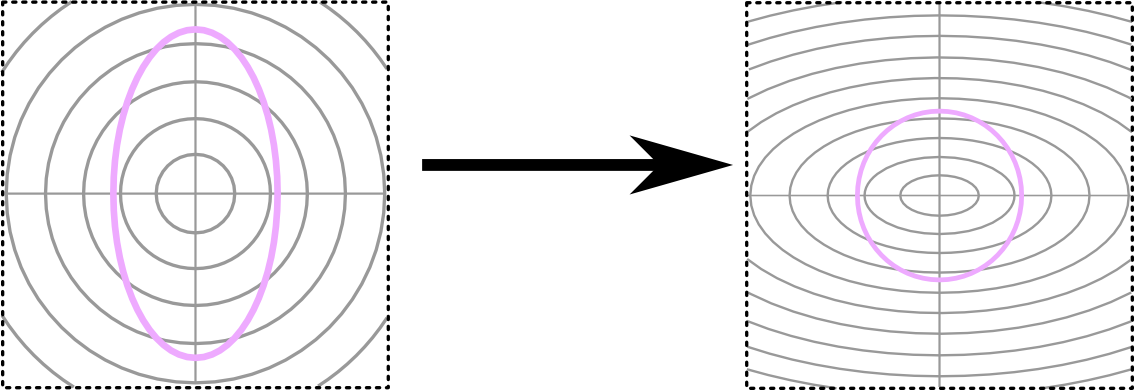
\includegraphics[width=0.8\textwidth]{fig/coordinate_transformation.png}
\label{fig:coord_trans}
\caption{A 2-dimensional linear coordinate transformation.}
\end{figure}

In order to apply the isotropic solution to this anisotropic case, we would like
to apply a coordinate transformation such that we can transform the problem into
an isotropic case with respect to some \(x' = a_x x\) and \(y' = a_y y\), as in
Figure \ref{fig:coord_trans}.
Without loss of generality, suppose \(a_x = 1\).

\begin{align}
\frac{dx'}{dx} &= 1\\
\frac{dy'}{dy} &= a_y\\
\frac{\partial f}{\partial x} &= \frac{\partial f}{\partial x'}\frac{dx'}{dx} = \frac{\partial f}{\partial x'}\\
\frac{\partial f}{\partial y} &= \frac{\partial f}{\partial y'}\frac{dy'}{dy} = a_y\frac{\partial f}{\partial y'}\\
\nabla T &= \frac{\partial T}{\partial x'} \e_{x'} + a_y\frac{\partial T}{\partial y'} \e_{y'} \\
[K]\nabla T &= k_x\frac{\partial T}{\partial x'} \e_{x'} + k_ya_y\frac{\partial T}{\partial y'} \e_{y'}\\
\nabla \cdot \left([K]\nabla T\right) &= k_x\frac{\partial^2 T}{\partial {x'}^2} + k_ya_y^2\frac{\partial^2 T}{\partial {y'}^2}\\
\end{align}

Suppose the right hand side is equal to the equivalent isotropic expression:
\begin{equation*}
k\left(\frac{\partial^2 T}{\partial {x'}^2} + \frac{\partial^2 T}{\partial {y'}^2} \right) = k_x\frac{\partial^2 T}{\partial {x'}^2} + k_ya_y^2\frac{\partial^2 T}{\partial {y'}^2}
\end{equation*}

As a result,

\begin{align*}
k &= k_x\\ a_y &= \sqrt{\frac{k_x}{k_y}}\\
\end{align*}

Therefore, the following coordinate transformation will allow us to apply the
isotropic solutions to an isotropic case with \(k = k_x\):

\begin{equation}
    \label{coord_trans}
    \begin{pmatrix}x' \\ y'\end{pmatrix} =
    \begin{bmatrix}1 & 0\\ 0 & \sqrt{\frac{k_x}{k_y}} \end{bmatrix}\begin{pmatrix}x \\ y\end{pmatrix}
\end{equation}

\section{From Temperature Distribution to Measurement}
\label{sec:analytical-np:isotropic}

Using equation \ref{coord_trans}, we may apply the isotropic solution:

\begin{equation}
    -k_x \nabla^2 T = \rho C\frac{\partial T}{\partial t}
\end{equation}

and get the following result (for sufficiently large \(t/r'\)):

\begin{equation}
T(r',t) = \frac{q}{4\pi k_x}\ln\left(\frac{4k_xt}{r'^2}\right) - \frac{\gamma q}{4\pi k_x}
\end{equation}

It is tempting to say that we're done here, but such is not the case. It can be
shown that, if \(r'\) is assumed to be a constant that ``falls out'' when 
differentiating as \(r\) is in the isotropic case that we are unable to recover
\(k_y\). In this case, we must also apply some other sort of transformation to
handle \(r'\) properly. This requires that we clarify exactly \emph{what} \(r\)
and \(r'\) mean in this context. When measuring for the anisotropic case, I
argue that we are effectively measuring the temperature at some
\(r = r_{\textrm{0}}\)---either on the surface of the needle, or some small
distance away from the needle.

This approach isn't without its problems. For example, it supposes that the
isotherms are all circles in the transformed geometry, but if a finite-sized
needle was actually being modeled in the problem then the isotherms near the
(elliptically-shaped in the transformed domain) needle would be elliptical as
well, and only isotherms sufficiently far away would be round. However, this
approach allows us to keep using the \(\ln()\) approximation, while a solution
given a finite needle would likely require the use of Bessel functions.

Applying this technique to the anisotropic case, we find that we must also
transform \(r_{xy} = \cos(\theta) \hat{e}_x + \sin(\theta) \hat{e}_y \)
into \(r_{x'y'}\):

\begin{align*}
    \begin{pmatrix}r_{x'} \\ r_{y'}\end{pmatrix} &=
    \begin{bmatrix}1 & 0\\ 0 & \sqrt{\frac{k_x}{k_y}} \end{bmatrix}\begin{pmatrix}r_0\cos(\theta) \\ r_0\sin(\theta)\end{pmatrix}\\
    &= r_0\left(\cos(\theta) \e_x + \sqrt{\frac1{k_y}} \e_y \right)\\
\end{align*}
\begin{equation}
    \norm{r'}^2 = r_0^2 \left(\cos^2(\theta) + \frac{k_x}{k_y}\sin^2(\theta) \right)\\
\end{equation}

This means that the temperature around the needle should now vary as a function
of \(\theta\), unlike in the isotropic case. Now, since the needle only measures
a single value, we may assume that the measured quantity is an
average temperature---say, the average surface temperature of the probe.  This
may be expressed like so:

\begin{equation}
\label{eq:tavg}
T_{\textrm{avg}}(t) = \frac{4\pi k_x}{q} \frac{\mathcal{E}(\ln(t), \frac{k_y}{k_x})}{\mathcal{E}(1, \frac{k_y}{k_x})}
\end{equation}

where:

\begin{equation}
\mathcal{E}(f(\phi, \alpha), \alpha) = \int_0^{2\pi} f\sqrt{\cos^2(\phi) + \alpha\sin^2(\phi)} d\phi
\end{equation}

\section{Finding Measured Conductivity as a Function of Needle Orientation}

In order to extract the measured \(k\) value, we fit a function of the form
\(C_1 \ln(t) + C_2\) to equation \ref{eq:tavg}. Then, all that is left is to evaluate the functions at various combinations of
\(k_xy\), \(k_z\) and \(\theta\).

\section{Software Implementation}

This method is implemented in python, in Appendix \ref{apx:analytical-np}. The ``elliptical'' and ``tavg'' functions to calculate theoretical long-time temperature curves as a function of time. The elliptical integrals are numerically evaluated using a quadrature method.  Then, the ``k\_meas'' function calculates the measured k-value that would result from a curve fit to the isotropic model. Finally, the ``\_\_main\_\_'' procedure calculates the resulting \(k\) measurements for various combinations of \(k_xy\), \(k_z\) and \(\theta\), and prints the results to stdout in .csv format so that a table of values may be generated and piped to a text file for future analysis.

\marginpar{Code snippets MAY be appropriate here.}

\section{Conclusions}
\label{sec:analytical-np:conclusion}

An analytical approach to studying anisotropic thermal conductivity with needle
probes is more difficult than with the isotropic case. However, by using
coordinate projections to pose the problem in two dimensions, and by applying
coordinate transformations to the domain, one may apply the accepted isotropic
theory to the anisotropic case with minimal modification.  By numerically
evaluating the predicted temperature distribution over time, one may find the
expected conductivity measurement given the theory holds for anisotropic
materials.

